%!TEX root = ../thesis.tex
\chapter{Background}
\label{ch:background}

This thesis integrates open problems in evolutionary biology with newly developed tools from applied topology.
As few readers are likely to have substantial exposure to both fields, we use this initial chapter to supply sufficient background to motivate later discussion.
Exposition required for specific results can be found in their respective individual chapters.

\section{Biology}

In this section we present biological background.
This section is intended to motivate the problems discussed.
More specific background relevant to the applications described in Part \ref{part:application_microorganism} and Part \ref{part:applications_human} is presented in those Parts.

What do we mean by horizontal and vertical evolution?
Vertical, or clonal, evolution is mediated by stochastic mutations over multiple generations.
Vertical evolution will be consistent with a phylogenetic tree.
Horizontal evolution...

\subsection{Evolutionary Processes}

Vertical: clonal.
Mutation and drift.
Horizontal; reticulate; lateral.
Recombination and reassortment.
Gene trees vs species trees.

\subsubsection{Genes and Genomes}

The information required for biological function is contained in an organisms genome.
The genome is the linear string of nucleotides that represent the set of genes in an organism.
Following the fundamental dogma of biology, DNA is transcribed into RNA, RNA is translated into amino acids, and amino acids are folded into proteins.
Proteins are the functional element of biology.

Beyond simply coding for an organisms function, the genome includes an imprint of the evolutionary history that gave rise to that particular organism.
Comparing the genomes of multiple organisms.
This is the field of \emph{comparative genomics}.

\subsubsection{Horizontal Gene Transfer}

Discussion of nonvertical evolutionary processes.
This will include references to Doolittle, Koonin, Gogarten.
Lateral Gene Transfer.
Species Trees and Gene Trees.
Recombination and reassortment.

\subsection{Mathematical Models of Evolution}
\label{background:ss:evolutionary_models}

Mathematical population genetics is concerned with properties of populations as they are subject to evolutionary forces over long time scales.
These forces include natural selection, genetic drift, mutation, and recombination.
Historically the input data for population genetics models was comparative studies of allele frequencies across populations.
Large-scale genome surveys.
Genealogy and population structure.

\subsubsection{The Wright-Fisher Model}

The Wright-Fischer model is a 
Forward time simulation of population.
Here we describe the simplest Wright-Fisher model: neutral, constant population size $N$.
At each time step randomly choose a parent.
\kje{[Figure comparing Wright-Fisher and Coalescent.]}

\subsubsection{The Coalescent Process}
\label{background:sss:coalescent}

The coalescent process is a stochastic model that generates the genealogy of individuals sampled from an evolving population \cite{Wakeley:2009}.
The genealogy is then used to simulate the genetic sequences of the sample.
This model is essential to many methods commonly used in population genetics.
Starting with a present-day sample of $n$ individuals, each individual's lineage is traced backward in time, towards a mutual common ancestor.
Two separate lineages collapse via a coalescence event, representing the sharing of an ancestor by the two lineages.
The stochastic process ends when all lineages of all sampled individuals collapse into a single common ancestor.
In this process, if the total (diploid) population size $N$ is sufficiently large, then the expected time before a coalescence event, in units of $2N$ generations, is approximately exponentially distributed:
\begin{equation}
P(T_{k}=t) \approx \binom{k}{2} e ^{-\binom{k}{2} t},
\end{equation}
where $T_k$ is the time that it takes for $k$ individual lineages to collapse into $k-1$ lineages.

After generating a genealogy, the genetic sequences of the sample can be simulated by placing mutations on the individual branches of the lineage.
The number of mutations on each branch is Poisson-distributed with mean $\theta t / 2$, where $t$ is the branch length and $\theta$ is the population-scaled mutation rate.
In this model, the average \emph{genetic distance} between any two sampled individuals, defined by the number of mutations separating them, is $\theta$.

The coalescent with recombination is an extension of this model that allows different genetic loci to have different genealogies.
Looking backward in time, recombination is modeled as a splitting event, occurring at a rate determined by population-scaled recombination rate $\rho$, such that an individual has a different ancestor at different loci.
Evolutionary histories are no longer represented by a tree, but rather by an \emph{ancestral recombination graph}.
Recombination is the component of the model generating nontrivial topology by introducing deviations from a contractibile tree structure, and is the component which we would like to quantify.
Coalescent simulations were performed using \texttt{ms} \cite{Hudson:2002}.

\subsubsection{Metrics on Sequences}

For the sequences from different organisms to be compared, they must first be aligned.
A sequence alignment is an arrangement of the characters in a set of sequences into a set of columns such that characters sharing evolutionary identity are in the same column.
In this case insertion and deletions can introduce gaps.
Alignment can be a complex part of any sequence analysis, particularly when there is substantial divergence between sequences of interest.
Performing sequence alignment is largely beyond the scope of this thesis, and in general we assume sufficient sequence similarity such that alignment can be performed without difficulty.

What metrics can we put on aligned sequences?
The simplest model, and the one most commonly adopted in this thesis, is the Hamming metric, which simply counts the differences.
Hamming metric: simple count of differences between

More biologically motivated metrics will incorporate some model of evolution and account for the possibility of back mutation.
These include Jukes-Cantor, Nei-Tamura, etc.

Jukes-Cantor metric is defined as 
\begin{equation}
d=-\frac{3}{4}\ln(1-\frac{4}{3}p).
\end{equation}

\subsection{Phylogenetic Reconstruction}

Phylogenetics is concerned with relationships among species as inferred from evolutionary characters.
In practice: tree-building.

Start with sequences.
Perform an alignment.
From an alignment, one can then directly use parsimony or likelihood approaches.
Alternatively, one can compute a matrix of pairwise distances and then construct a tree that best approximates these distances.
Most relevant to this thesis are the distance-based approaches (because they can be viewed as finite metric spaces amenable to topological analysis).
Only in the case of perfectly additive data will a tree be able to exactly fit the matrix.
Identifying the pairwise distance matrix with a its finite metric space representation allows most of the results described here.

Include discussion of rooted vs unrooted.

\subsubsection{Distance Matrix Methods}

Introduced by Cavalli-Sforza and Edwards in 1967 \cite{CavalliSforza:1967th} and Fitch and Margoliash in 1967 \cite{Fitch:1967we}.
Compute a matrix of pairwise distances and then find the tree that best approximates those distances.
Weighted and unweighted least squares.
UPGMA.
Neighbor joining is now the most common distance-matrix approach because it can perfectly reconstruct an additive tree.
Neighbor joining was introduced by Saitou and Nei in 1987 \cite{Saitou:1987wo}.

There are limitations of distance based methods.
Do not use all the information.

Need to include discussion of metrics on aligned sequences.

\subsubsection{Phylogenetic Networks}

Several existing methods for representing reticulate evolution.
Most assume the simplest generalization.
However, the resulting networks can be complex and difficult to interpret quantitatively.
Split Networks.
(Look at Morrison Review.)

\subsubsection{Space of Phylogenetic Trees}

Studies of tree space were initiated by Billera, Holmes, and Vogtmann in \cite{Billera:2001tv}.
Tree space on $L$ leaves is modeled as a subspace of $\mathbb{R}^{(XX)}$, where 
In their model, each point represents an unrooted binary tree with $L$ leaves and positive branch lengths.
Number of interior edges $r=L-3$, a particular additive tree can be plotted as a point in the positive open orthant $(0,\infty)^{r}$.
A single orthant corresponds to a single tree topology.
[Include treespace figure].

\subsubsection{Number of Trees}

The number of unrooted bifurcating tree topologies with $L$ leaves is $(2L-5)!!$.
This can be most easily seen via induction.
For $L=3$ leaves there is $1$ unrooted tree topology and $3$ line segments.
To move to the case of $L=4$, we can add the fourth leaf to any of the $3$ segments.
This results in $3$ possible topologies with $5$ total line segments (4 external leaves and 1 internal segment).



The number of rooted bifurcating tree topologies with $L$ leaves is $(2L-3)!!$
The number of unrooted bifurcating tree topologies with $L$ leaves is $(2L-5)!!$.
As can be seen, the number of tree topologies explodes with the number of leaves.
Fitch quote: \emph{more than 20 species, more than Avogadro's number of topologies.}
Phylogeny can be seen as projecting onto the space of trees.

%%%%%%%%%%%%%%%%%%%%%%%%%%%%%%%%%%%%%%%%%%%%%%%%%%%%%%%%%%%%%%%%%%%%%%%%%%%%%%%%%%%%%%%%%%%%%%%%%%%%
%%%%%%%%%%%%%%%%%%%%%%%%%%%%%%%%%%%%%%%%%%%%%%%%%%%%%%%%%%%%%%%%%%%%%%%%%%%%%%%%%%%%%%%%%%%%%%%%%%%%

%%%%%%%%%%%%%%%%%%%%%%%%%%%%%
% TOPOLOGICAL DATA ANALYSIS %
%%%%%%%%%%%%%%%%%%%%%%%%%%%%%

\section{Topological Data Analysis}

\subsection{Intuition}

\subsection{Constructing Spaces from Real Data}

With a metric we can represent this as a finite metric space.
How can we apply the ideas of topology to these spaces?

\paragraph{Finite Metric Spaces}

Finite metric spaces are really interesting objects of study.
Lots of good work on embedding finite metric spaces, see Matousek.
Metric space with a finite number of points.
Combinatorics, geometric, and algorithms.
In topological data analysis, our spaces of interest are finite metric spaces.

\subsubsection{The \Cech\ and Vietoris-Rips Complexes}

The \Cech\ complex consists of the set of simplices $\sigma$ with vertices $v_{1},...,v_{k}\in S$ such that

\begin{equation}
\displaystyle\cap_{i}^{} B(v_{i},\epsilon)\neq0
\end{equation}

The Vietoris-Rips complex is defined as

\begin{equation}
\mathrm{VietorisRips}(r) = \{ \sigma\in S\:|\:\mathrm{diam}(\sigma) \leq 2r \}
\end{equation}
where $\mathrm{diam}(\sigma)=\{ \sup d(i,j) \:|\: i,j\in\sigma \}$

\subsubsection{Filtrations}

A series of inclusions.

\subsection{Condensed Representations}

\subsubsection{The Mapper Algorithm}
\label{subsec:mapper}

Condensed Representations.
Exploratory data analysis seeks to represent high-dimensional datasets in .

\begin{figure}
\begin{tikzpicture}[node/.style={minimum height=.8cm,minimum width=2cm,draw}]
\draw (0,0) node[node, align=center] (dr) {Dimensionality\\Reduction};
\draw (3,1) node[node] (linear) {Linear};
\draw (3,-1) node[node] (nonlinear) {Nonlinear};
\draw (6,1) node[node] (pca) {PCA};
\draw (6, -.5) node[node] (geometry) {Geometry};
\draw (6, -1.5) node[node] (topology) {Topology};
\draw (9, -.5) node[node,align=left] (manifold_learning) {Manifold\\Learning};
\draw (9, -1.5) node[node] (mapper) {Mapper};
\draw (12, -.5) node[node,align=center] (mds) {MDS\\PCA\\Isomap};


\myline{dr}{linear};
\myline{dr}{nonlinear};
\draw[-latex] (linear) -- (pca);
\myline{nonlinear}{geometry};
\myline{nonlinear}{topology};
\draw[-latex] (topology) -- (mapper);
\draw[-latex] (geometry) -- (manifold_learning);
\draw[-latex] (manifold_learning) -- (mds);

\end{tikzpicture}
\caption[Dimensionality Reduction for EDA]{Dimensionality Reduction for EDA}
\label{background:fig:eda}
\end{figure}


Mapper algorithm was first developed in \cite{Singh:2007ve}.
Mapper is coordinate free and depends onnly on the similarity of points as measured by the distance function.
Further exposition can be found in \cite{Lum:2013cz}.
Used in biology example in \cite{Nicolau:2011} top classify breast cancer subtypes.
In our work we use the commercial Mapper implementation Ayasdi \cite{AyasdiIris:2015}.
An open-source implementation of the Mapper algorithm is avvailable in the Python Mapper package \cite{Mullner:2013}.

Steps:
(1) Project using filter function.
(2) Create overlapping bins
(3) Cluster in the projected space.
(3) Connect pairs of bins with shared points

\subsection{Persistent Homology}
\label{background:ss:persistent_homology}

How to extend homology to finite metric spaces?

From the point cloud, a nested family of simplicial complexes, or a filtration, is constructed, parameterized by a filtration value $\epsilon$, which controls the simplices present in the complex.
The two most common ways of constructing a simplicial complex at each $\epsilon$ are the \Cech complex and the Vietoris-Rips complex.
The filtration is represented as a list of simplices defined on the vertices of $S$, annotated with the $\epsilon$ at which the simplex appears.
Given a filtration, the persistence algorithm is used to compute homology groups.
The $0$-dimensional homology ($H_0$) represents a hierarchical clustering of the data.
Higher dimensional homology groups represent loops, holes, and higher dimensional voids in the data.
Each feature is annotated with an interval, representing the $\epsilon$ at which the feature appears and the $\epsilon$ at which the feature contracts in the filtration.
These filtration values are the \emph{birth} and \emph{death} times, respectively.



\begin{figure}
\centering
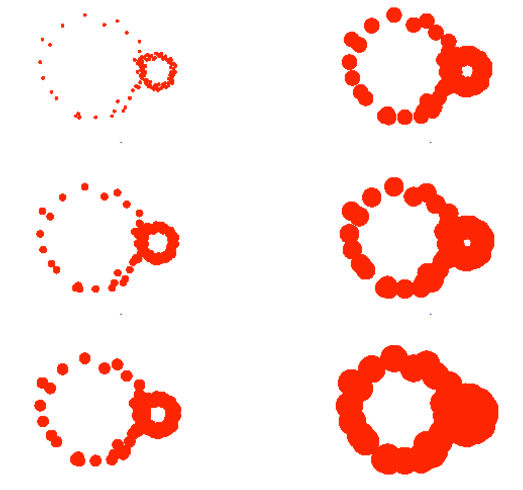
\includegraphics[]{./fig/LESNICK_ExpandingBalls.pdf}
\caption[A filtration]{Example of constructing a filtration.}
\label{background:fig:exanding balls}
\end{figure}

\begin{figure}
\centering
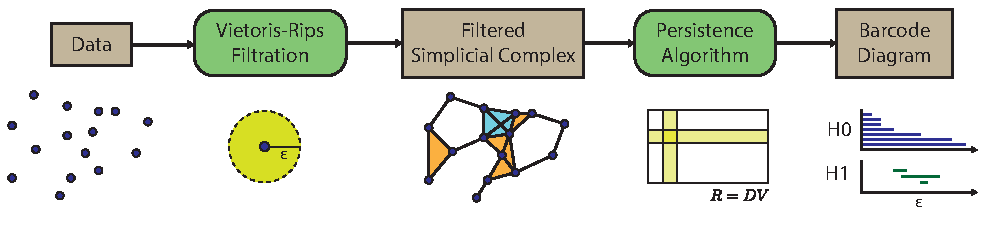
\includegraphics[]{./fig/persistence_pipeline.pdf}
\caption[The Persistence Pipeline]{The Persistence Pipeline.}
\label{background:fig:persistence_pipeline}
\end{figure}

\subsubsection{The Persistence Algorithm}
\label{subsubsec:ph_algorithm}

While we act mostly as an end-user of persistent homology in this thesis, the algorithmics behind efficient computations of homology are interesting and worth including for comprehensiveness.
Computing persistent homology is an exercise in linear algebra.
The initial algorithms first induce a matching on a set of simplices.
This is due to Zomorodian and is the implementation used in Javaplex and Dionysus.
Then you reduce a couple of matrices.
You can read off each bar and its represetnative cycle from looking at the zeros on this one particular matrix.
Smith normal form.

More advanced algorithms have been developed that compute simplicial collapses: recognizing that the size of the simplciial set is often the limiting factor here, they collapse simplicies into simpler structures that will have identical homology.
This uses Discrete Morse Theory and is the idea behind implementations such as Perseus.

Include only simple implementation for $Z2$.

Several packages for computing persistent homology have been developed [Dionysus, Javaplex, Guidi, phom] and TDA frontend for R.
Persistent homology is computed using Dionysus \cite{Morozov:2012}.

\subsubsection{Stability}
\label{subsubsec:ph_stability}

An important aspect of peristent homology is stability.
Stability refers to how the output of persistent homology will change when the original data is perturbed, for example due to noise or sampling.
Will the existing bars change?
Will new homology classes be formed?
We would like the output of persistent homology to be stable under these perturbations.
In general, our question is if I have some perturbation that takes my data from $D\rightarrow D'$, what can I say about the subsequent change in barcodes $B\rightarrow B'$?
In general, if I have data $D$ that is perturbed to new data $D'$, how will change
Luckily, there is a result that bounds changes in the diagram, due to Chazal and coauthors \citep{Chazal:2009wc}.
After a few definitions, we state the stability theorem.
First, we consider metrics on spaces.

\begin{defn}
\label{defn:hausdorff}
The \emph{Hausdorff distance} measures the distance between two shapes.
\begin{equation}
d_{H}(X,Y) = \max\left\{ \sup_{x \in X} \inf_{y \in Y} d(x,y), \sup_{y \in Y} \inf_{x \in X} d(X,Y) \right\}
\end{equation}
And $d_H(X,Y)=0$ iff $X=Y$.
\end{defn}

\begin{defn}
\label{defn:gromovhausdorff}
The \emph{Gromov-Hausdorff distance} measures how far two spaces are from being isometric.
It measures the longest distance from a point in one set to the closest point in another set within a metric space.
\begin{equation}
d_{GH}(X,Y)=\inf_{f,s} d_H(X,Y)
\end{equation}
\end{defn}

Next, we consider how to define the distance between two persistance diagrams.
To do so, we first need the concept of a \emph{matching}.
For two persistence diagrams $A$ and $B$, a matching is a mapping from intervals in $A$ to intervals in $B$, where we allow points to match to the diagonal to account for cases with unequal number of points.
For each matched pair of intervals $(a,b)$, we define the $L_{\infty}$ distance as

\begin{equation}
d_{\infty}(a,b) = \max\{ |a_{x}-b_{x}|, |a_{y}-b_{y}| \}.
\end{equation}


\begin{defn}
\label{defn:bottleneck}
The \emph{bottleneck cost} of a matching between two diagrams is the maximum $L_{\infty}$ for all matched points. The \emph{bottleneck distance} is defined to be the minimal bottleneck cost across all matchings. The matching with minimal bottleneck cost is the \emph{bottleneck matching}.
\begin{equation}
d_{B}(A,B) = \inf_{n:A\rightarrow B} \sup_{x\in X} ||x-\eta(x)||_{\infty}
\end{equation}
\end{defn}

The result of \citet{Chazal:2009wc} states that the bottleneck distance between $B$ and $B'$ is bounded by the Gromov-Hausdorff distance between the finite metric spaces embedded in $A$ and $B$.

\begin{thm}
\label{thm:stability}
The stability theorem.
\begin{equation}
d_{B}(H_{K}(X),H_{K}(Y)) \leq d_{GH}(X,Y)
\end{equation}
\end{thm}

This bound establishes that small perturbations in the data will produce only small changes in the the persistence diagram.

\subsubsection{Statistical Persistent Homology}
\label{subsubsec:ph_statistics}

In persistent homology, the intuition is developed that long intervals are to be interpreted as large-scale, or robust, geometric features in data, while short intervals are more likely to correspond to noise or incomplete sampling.


More broadly, how can the information in the persistent diagram be used 
Can this statement be made more precise?
How short is short, and how will noisy sampling effect the observed diagram?
When can a long interval be interpreted as a real feature, and can we assign measures of confidence to our estimates?
Substantial recent work in the TDA community has focused on these questions, in order to develop statistical foundations for persistent homology.
We give here a brief flavor of some of these ideas and their relation to our own work.

Fasy and coauthors have developed ways of generating confidence intervals for persistence diagrams \citep{Fasy:2014}.
Based on some information about density, they can put a line off the diagonal below which points are to be considered noise (see example).
Bubenik has developed the language of persistence landscapes \cite{Bubenik:2007ux,Bubenik2015:um}.  
Several authors have examined the space of persistence diagrams as a Polish space, with notions of mean and variance.
XXX et al have used the bootstrap to get estimates of the diagram robustness.
Mukherjee et al.

Also see the work of Turner \cite{Turner:2012wb} and Mileyko \cite{Mileyko:2011jm}.

\begin{itemize}
\item Probability measures on the space of persistence diagrams
\item Functional summaries of the persistence diagram
\item Confidence intervals on the persistence diagram
\item Statisical inference using persistence diagrams
\item 
\end{itemize}

Wasserstein distance between diagrams.

\begin{equation}
W_{p}(D_{1},D_{2}) = \left( \inf_{\gamma} \sum_{x\in D_1} \|x-\gamma(x)\|^{p}_{\infty} \right)^{1/p}
\end{equation}

\kje{[Expand substantially, this section needs to be very strong.]}

\subsubsection{Multidimensional Persistence}
\label{subsubsec:ph_multidim}

First laid out in \cite{Carlsson:2009b}.
More work in \cite{Lesnick:2012uv}.
Filtrations along different dimensions; how to relate?.
Prototypical example: density and distance.

Our case is going to be slightly different.
We will consider a set of points annotated with different metrics that we can put on it which will induce different homologies.
Then we will see what happens we interpolate between those different metrics.
\kje{[Discuss with Michael.]}

%%%%%%%%%%%%%%%%%%%%%%%%%%%%%%%%%%%%%%%%%%%%%%%%%%%%%%%%%%%%%%%%%%
%% Applying TDA to Molecular Sequence Data
%%
%% Mapper and Persistent Homology?
%%
%%%%%%%%%%%%%%%%%%%%%%%%%%%%%%%%%%%%%%%%%%%%%%%%%%%%%%%%%%%%%%%%%%

\section{Applying TDA to Molecular Sequence Data}

Aligned genomic sequences can be naturally viewed as points in a high-dimensional sequence space.
As more genomes continue to be sequenced, this space becomes more densely sampled.
Using the standard genetic distance metrics described above, we can compute a pairwise distance matrix betwee genomes.
This defines our finite metric space.
From there, methods from TDA can be applied.
In particular, we can apply persistent homology, and phylogenetic information contained in the dataset can be read off the resulting barcode diagram.

An important foundational point was described in \cite{Chan:2013}.
In that paper, it was shown that if the evolutionary history contained in a particular data-set is tree-like, then there will be no higher homology in the resulting barcode diagram.
In other words, the only nontrivial topology will appear in dimension zero.

If the set of genomes permits a phylogenetic representation, then positive-dimensional Betti numbers should vanish, since the topology of a tree is contractible. 
\kje{[More about Gunnar's proof?]}
If the evolutionary history includes reticulate events that cannot be represented as a tree, these events will be captured as non-trivial higher dimensional homology in the barcode diagram.

We illustrate a simple example of how TDA can capture horizontal evolution from populaton data in Figure~\ref{background:fig:tda_on_sequencedata}.
Consider the reticulate phylogeny (Figure~\ref{background:fig:tda_on_sequencedata}A): five genetic sequences sampled today (yellow circles) originate from a single common ancestor due to clonal evolution (solid blue lines tracing parent to offspring) and reticulate evolution (dotted red lines).
In Figure~\ref{background:fig:tda_on_sequencedata}B, these five samples are placed in the context of a larger dataset, where the data has been projected onto the plane using PCA.
Persistent homology is then applied to this larger sample.
In Figure~\ref{background:fig:tda_on_sequencedata}C we demonstrate the construction of a filtered simplicial complex, showing how the connectivity changes as the scale parameter $\epsilon$ is increased.
Finally, in Figure~\ref{background:fig:tda_on_sequencedata}D we see the resulting barcode diagram.
Using $H_0$ we can track the number of strains or subclades that persist, roughly corresponding to the tree-like component of the data.
The $H_1$ bar near spanning roughly $\epsilon=0.13$ to $\epsilon=0.16$ identifies the presence of a reticulate event. involving the five higlighted sequences.
The scale over which this bar persists represents the amount of evolutionary time separating the parents and the reticulate offspring.
Additionally, the persistence algorithm will return a generating basis for a particular homology group, which we can use to identify the particular mixtures of sequences involved a reticulation.
In this way, we can analyze both the scale and frequency of reticulation in genomic data sets.

We summarize the connection between genomics and TDA in Table~\ref{table:dictionary}.

\begin{table}
\centering
\caption{Dictionary connecting algebraic topology and evolutionary biology}
\small
\rowcolors{2}{gray!25}{white}
\setlength{\aboverulesep}{0pt}
\setlength{\belowrulesep}{0pt}
\setlength{\extrarowheight}{.75ex}
\begin{tabularx}{\textwidth}{XX}
\toprule\rowcolor{gray!50}
Algebraic Topology                                         & Evolutionary Biology \\
\midrule
Filtration value $\epsilon$                                & Genetic distance (evolutionary scale) \\
0-dimensional Betti number at filtration value $\epsilon$  & Number of clusters at scale $\epsilon$ \\
Generators of 0-D homology                                 & A representative element of the cluster \\
Hierarchical relationship among generators of 0-D homology & Hierarchical clustering \\
1-D Betti number                                           & Lower bound on number of reticulate events \\
Generators of 1-D Homology                                 & Reticulate events \\
Generators of 2-D Homology                                 & Complex horizontal genomic exchange \\
Non-zero high-dimensional homology (“topological obstruction to phylogeny”) & No treelike phylogenetic representation exists \\
Number of higher-dimensional generators over a time interval (“irreducible cycle rate”) & Lower bound on recombination/reassortment rate \\
\bottomrule
\end{tabularx}
\label{table:dictionary}
\end{table}

\begin{figure}
\centering
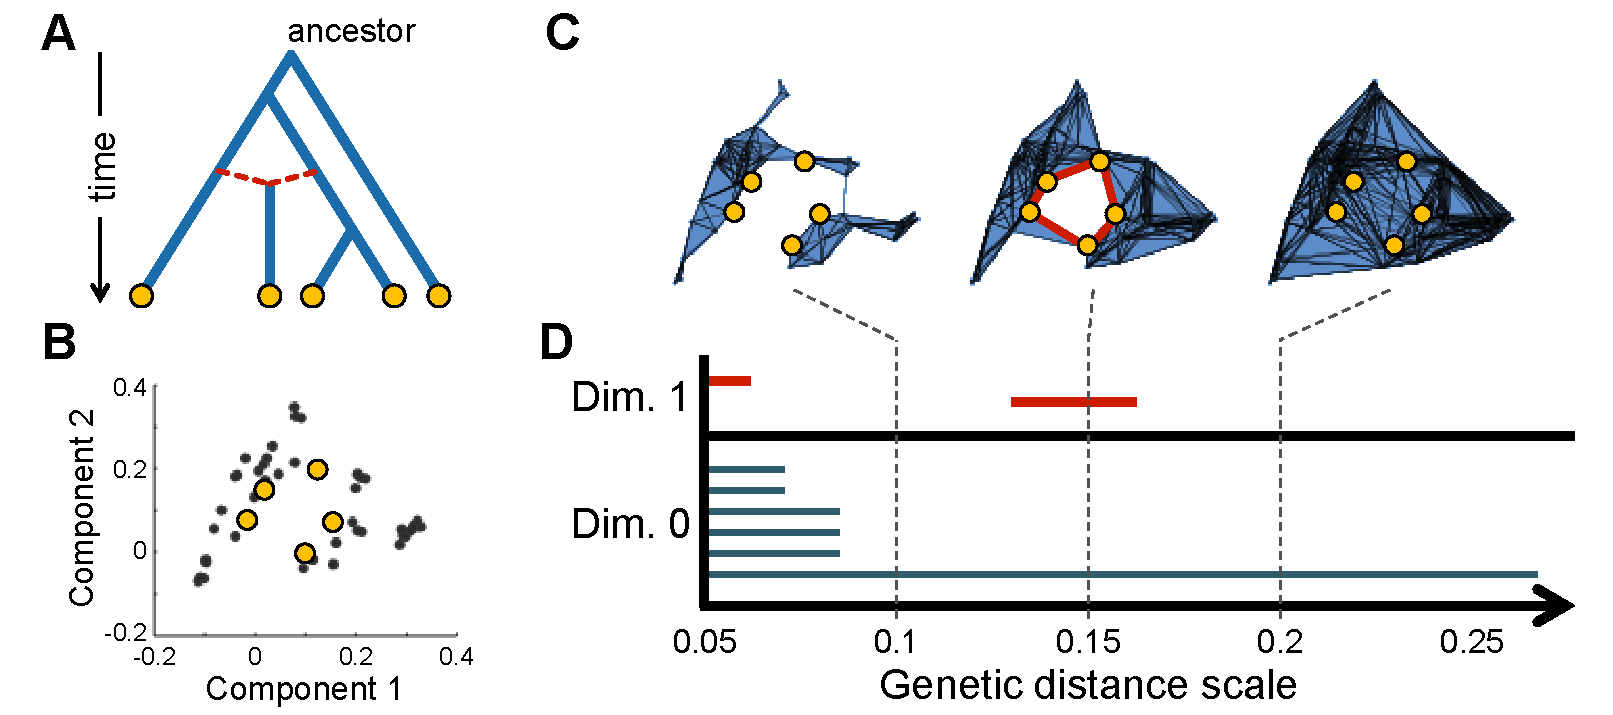
\includegraphics[width=\textwidth]{./fig/tda_on_sequencedata.pdf}
\caption[Applying TDA to Sequence Data]{Applying persistent homology to genomic data. (A) An evolutionary genealogy including reticulation. (B) Data projected into 2-dimensions. (C) Construction of a filtered simplicial complex. (D) The resulting multiscale barcode diagram.}
\label{background:fig:tda_on_sequencedata}
\end{figure}

\subsection{The Simplest Example}

Recall the four gamete test, which tests for the prescence of reticulate evolution by searching for the simultaneous presence of 
Recall the four gamete test.
The simplest example is 00, 10, 01, 11.
Under a Hamming metric this forms a loop.

\subsection{The Space of Trees, Revisited}

Recall our description of the space of trees in Section~XX.
There, we made reference to the idea that the goal of phylogenetic reconstruction can be seen as finding the best projection onto tree space for some arbitrary dataset.
Expand our search space.
New goal is to characterize the space of finite metric spaces.
As we move off tree space, we know there is no additive tree that represents the data.
Then we want some topological measure of deviation from additivity.
So our updated picture looks like Figure~XX.

